\chapter{Tag 16 — Wenn ECC die Welt rettet}

\begin{quote}
Du hast den Encoder gebaut, du hast Dein Symbol von Hand gezeichnet,
Du hast die Klassenhierarchie aufgeräumt — und an einer Stelle hast
Du immer wieder Vertrauensvorschuss gegeben: dass die Reed-Solomon-
Prüfbytes wirklich Fehler reparieren. Heute kassieren wir diesen
Vorschuss ein. Wir bauen einen Decoder, der nicht nur den Klartext
zurückliefert, sondern auch sagt, \emph{wo} der Schaden war —
und füttern ihn dann mit absichtlich beschädigten Symbolen.
\end{quote}

\section*{Lernziele für heute}

Am Ende von Tag 16 kannst du \dots

\begin{itemize}
\item den Decoding-Datenfluss erklären: Bild $\to$ Modul-Matrix
  $\to$ Codewords $\to$ Reed-Solomon-Korrektur $\to$ Klartext
\item die inverse Datenplatzierung von Etappe 13 nutzen, um aus
  einem Symbol die ursprünglichen Codewords zurück­zugewinnen
\item \texttt{reedsolo} mit dem Datamatrix-Polynom anwenden und
  die Fehler-Position aus dem Decoder-Ergebnis lesen
\item kaputte Module im Symbol farblich markieren und so die
  Wirkung der Reed-Solomon-Korrektur visuell zeigen
\item empirisch ermitteln, ab welcher Fehlerzahl der Decoder
  versagt — und das Ergebnis mit der theoretischen RS-Grenze
  vergleichen
\end{itemize}

\paragraph{Material} Laptop mit Thonny, \texttt{reedsolo} aus
Etappe 8, dein Datamatrix-Encoder aus Etappe 15, dein hand­gezeichnetes
\texttt{GRETA}-Symbol von Tag 13 und etwas Tipp-Ex (oder einen dicken
schwarzen Filzstift).

% =============================================================
\section{Was ein Decoder eigentlich macht \normalfont(\textit{≈ 10 min})}
% =============================================================

Encoding war ein Pfeil von links nach rechts:
\begin{center}
\texttt{Klartext $\to$ ASCII$+$1 $\to$ RS-ECC $\to$ Datenplatzierung $\to$ Frame $\to$ PNG}
\end{center}

Decoding ist genau der umgekehrte Weg — mit einer entscheidenden
Wendung in der Mitte:
\begin{center}
\texttt{PNG $\to$ Modul-Matrix $\to$ Codewords $\to$ \textbf{RS-Korrektur} $\to$ Klartext}
\end{center}

Im Encoder war der RS-Schritt nur „berechne die Prüfbytes und hänge
sie an". Im Decoder ist der RS-Schritt der spannende: er erkennt,
dass einige Codewords nicht mehr zu den Prüfbytes passen, lokalisiert
den Fehler und korrigiert ihn.

\subsection*{Inverse Datenplatzierung}

Aus Etappe 13 hast du eine Funktion \texttt{place\_codewords}, die
aus 12 Codewords eine 12$\times$12-Modul-Matrix macht. Heute brauchst
du den umgekehrten Weg: aus einer Modul-Matrix wieder 12 Codewords.

Der Trick: \texttt{\_build\_layout} liefert für jedes Datenmodul ein
Paar \texttt{(codeword\_nr, bit\_nr)}. Wir laufen das Layout ab, lesen
für jedes Modul den 0/1-Wert aus der Matrix und sammeln pro Codeword
die acht Bits zu einem Byte. Bit 1 ist das MSB (Wert 128), Bit 8 das
LSB (Wert 1) — wie immer.

% =============================================================
\section{Den DatamatrixDecoder bauen \normalfont(\textit{≈ 25 min})}
% =============================================================

\begin{pythoneinheit}{1}{Decoder-Klasse: Konstruktor, Bild-Sampling, Codewords}
\pythoncodeteil{tag16/decoder.py}{klasse}

Drei Dinge zum Mitschauen:

\begin{itemize}
\item \texttt{from\_png} ist ein \emph{Klassenmethode} — sie liefert
  eine fertige Instanz aus einer Datei. Konvention: Klassenmethoden
  starten oft mit \texttt{from\_\dots}.
\item \texttt{\_matrix\_zu\_codewords} läuft die Layout-Tabelle ab
  und sammelt pro Codeword die acht Bits. Identische Logik wie in
  Etappe 13, nur in die andere Richtung.
\item \texttt{\_rs\_decodieren} nutzt \texttt{reedsolo} mit den
  Datamatrix-spezifischen Parametern \texttt{prim=0x12D},
  \texttt{generator=2}, \texttt{fcr=1}. Das matcht das Polynom aus
  Etappe 12 — sonst gäbe es Inkompatibilitäten.
\end{itemize}

Die wichtigste Eigenschaft: \texttt{rs.decode(\dots)} liefert ein
Tripel \texttt{(daten, daten\_mit\_ecc, errata\_pos)}. \texttt{errata\_pos}
ist genau das, was wir wollten: die Liste der 0-basierten Indizes,
wo der Decoder Fehler gefunden hat.
\end{pythoneinheit}

\begin{bleistiftuebung}{1}{Inverse Place verstehen}
Nimm dir das vorbefüllte HONIG-Symbol vom Werkstattbogen (Etappe 13).
Wähle ein beliebiges Datenmodul aus — z.\,B. \texttt{(zeile, spalte)
= (3, 7)}. Was sagt dir das Layout: \emph{welches Codeword} und
\emph{welches Bit dieses Codeworts} steht an dieser Stelle?

Tipp: \texttt{\_build\_layout(10)} liefert für die 10$\times$10-Innen­fläche
die \texttt{(cw, bit)}-Zuordnung. In Thonny kannst du das in der
Shell direkt aufrufen.
\end{bleistiftuebung}

% =============================================================
\section{Fehler hineinkippen — und sehen, was passiert \normalfont(\textit{≈ 15 min})}
% =============================================================

\begin{pythoneinheit}{2}{Visualisierung: kaputte Module rot überlagern}
\pythoncodeteil{tag16/decoder.py}{visualisierung}

Wir nehmen das Symbol-PNG, legen ein halbtransparentes rotes Overlay
darüber und zeichnen für jedes Modul, das zu einem als kaputt
erkannten Codeword gehört, ein Quadrat. Das Ergebnis sieht etwa so
aus:
\end{pythoneinheit}

\begin{center}

\includegraphics[width=0.42\linewidth]{abbildungen/tag16/greta_beschaedigt_markiert.png}
\end{center}

Wir hatten in diesem Beispiel drei zufällige Datenmodule per
Bit-Flip kaputtgemacht. Was du jetzt siehst, ist mehr: alle Module,
die zum gleichen \emph{Codeword} gehören wie ein kaputter Modul,
sind rot markiert. Die kompakte L-Form jedes Codeword-Blocks (die
„Utah" aus Etappe 13!) wird so zum ersten Mal als zusammen­hängende
Einheit sichtbar — vier rote Cluster für vier betroffene Codewords.

\begin{bleistiftuebung}{2}{Vorhersage und Test}
\textbf{Bevor du den Code laufen lässt:} kippe in deinem
\texttt{GRETA}-Symbol in Gedanken die Module \texttt{(2, 5)},
\texttt{(4, 3)} und \texttt{(7, 8)}. Wieviele \emph{Codewords} werden
dadurch beschädigt? (Die Antwort kannst du nicht ohne das Layout
ablesen — aber rate.) Lass den Decoder laufen und vergleiche.
\end{bleistiftuebung}

% =============================================================
\section{Stress-Test: wie viele Fehler hält RS aus? \normalfont(\textit{≈ 20 min})}
% =============================================================

Reed-Solomon hat eine harte theoretische Grenze:
\begin{quote}
Mit $t$ ECC-Codewords lassen sich bis zu $\lfloor t/2 \rfloor$
Codewort-Fehler korrigieren.
\end{quote}

Bei einem 12$\times$12-Symbol mit 7 ECC-Codewords sind das also
3 Codewort-Fehler. Aber: ein einzelner Modul-Flip macht ein Codeword
kaputt; zwei Modul-Flips können ein oder zwei Codewords betreffen,
je nachdem, ob sie im selben Utah-Block landen oder nicht. Wir haben
also kein einfaches „bis zu 3 Modul-Flips" — sondern eine
Wahrscheinlichkeitsverteilung.

\begin{pythoneinheit}{3}{Experiment: Erfolgsquote messen}
\pythoncodeteil{tag16/fehler_demo.py}{experiment}

Wir flippen \texttt{anzahl} zufällig ausgewählte Datenmodule
(Frame-Module bleiben unangetastet — wer das L-Pattern kaputt macht,
hat sowieso verloren) und schicken die kaputte Matrix durch den
Decoder. \texttt{seed=42} sorgt dafür, dass das Experiment
reproduzierbar ist — gleiche Zahlen kommen jedes Mal raus.
\end{pythoneinheit}

\begin{pythoneinheit}{4}{Diagramm zeichnen}
\pythoncodeteil{tag16/fehler_demo.py}{diagramm}

\textbf{Neue Bibliothek: \texttt{matplotlib}.}
\texttt{matplotlib} ist \emph{die} Standard-Bibliothek für
Diagramme in Python — Linien, Balken, Kurven, alles. Installation
einmalig in Thonny über \textit{Tools → Manage packages}
oder im Terminal:

\begin{minted}{text}
pip install matplotlib
\end{minted}

Im Skript passieren drei Dinge:

\begin{itemize}
\item \texttt{fig, ax = plt.subplots(...)} legt eine neue
  „Leinwand" (\texttt{fig}) mit einem Koordinatensystem
  (\texttt{ax}) an. \texttt{figsize} steuert Breite und Höhe
  in Zoll.
\item \texttt{ax.plot(xs, ys, "b-o")} zeichnet die blaue
  Kurve: blaue Farbe (\texttt{b}), Linie (\texttt{-}),
  Kreispunkte (\texttt{o}).
\item \texttt{fig.savefig("...\,.pdf")} speichert als
  druckfähige Vektorgrafik — kein Pixelmatsch beim Zoomen.
  Eine senkrechte rote Linie markiert die theoretische
  RS-Grenze.
\end{itemize}
\end{pythoneinheit}

\begin{pythoneinheit}{5}{Demo: Erfolgsquote für GRETA in 12$\times$12}
\pythoncodeteil{tag16/fehler_demo.py}{demo}

Erwartete Konsolen-Ausgabe (200 Versuche pro Stufe, Seed 42):

\begin{minted}{text}
   0 Modul-Flips: 100.0%  ##############################
   1 Modul-Flips: 100.0%  ##############################
   2 Modul-Flips: 100.0%  ##############################
   3 Modul-Flips: 100.0%  ##############################
   4 Modul-Flips:  45.5%  ##############
   5 Modul-Flips:  16.5%  #####
   6 Modul-Flips:   3.5%  #
   7 Modul-Flips:   0.0%
\end{minted}

Und das Diagramm:
\end{pythoneinheit}

\begin{center}
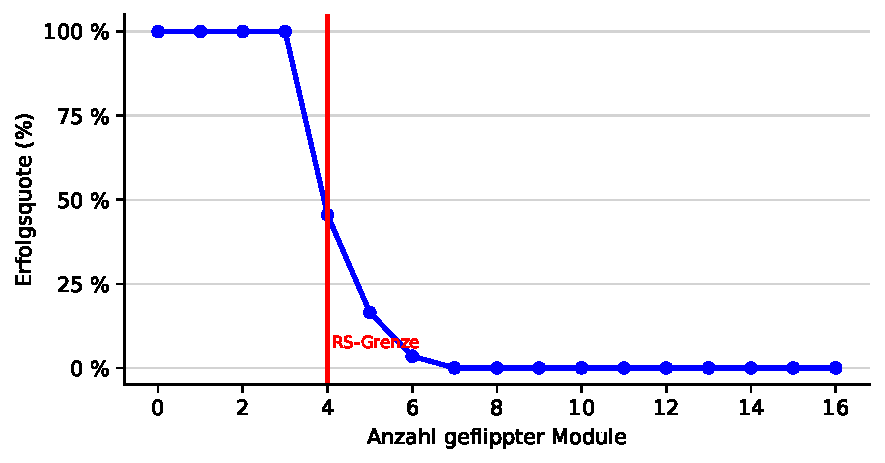
\includegraphics[width=0.85\linewidth]{abbildungen/tag16/fehler_demo_diagramm.pdf}
\end{center}

Lies die Kurve so:

\begin{itemize}
\item Bis \textbf{drei} Modul-Flips ist der Decoder unbestechlich.
  Diese Flips betreffen je 1--3 verschiedene Codewords; der
  RS-Decoder schluckt das.
\item Bei \textbf{vier} Modul-Flips fällt die Erfolgsquote schlag­artig
  auf etwa 45\,\%. Genau das ist der Punkt, an dem die zufälligen
  Flips öfter mal vier verschiedene Codewords erwischen — und damit
  über die theoretische RS-Grenze gehen.
\item Bei \textbf{sieben} Flips ist die Sache vorbei. Der Decoder
  versagt zuverlässig.
\end{itemize}

\begin{bleistiftuebung}{3}{Hand-Symbol mit Tipp-Ex}
Nimm dein hand­gezeichnetes \texttt{GRETA}-Symbol vom Werkstattbogen
aus Tag 13 und übermale gezielt einzelne Module mit Tipp-Ex (weiß)
oder einem schwarzen Filzstift. Fang mit einem Modul an, scanne mit
deinem Handy. Klappt's? Mach ein zweites kaputt, scanne wieder.
Steigere langsam — du solltest empirisch ungefähr die gleiche
Grenze finden wie das Python-Experiment.

Tipp: ändere möglichst \emph{Datenmodule}, nicht das L-Pattern oder
das Zeitsignal — die werden zum Lokalisieren des Symbols gebraucht
und sind nicht vom RS-Decoder gedeckt.
\end{bleistiftuebung}

% =============================================================
\section{Reflexion und Brücke zu Tag 17 \normalfont(\textit{≈ 10 min})}
% =============================================================

Du hast jetzt den vollen Kreis geschlossen:

\begin{itemize}
\item Du kannst Datamatrix-Symbole \emph{kodieren} (Etappen 11--15)
  — vom Klartext bis zum scannbaren PNG, in einer Klassenhierarchie.
\item Du kannst Datamatrix-Symbole \emph{dekodieren} (heute) —
  inklusive Fehler-Lokalisation.
\item Du hast empirisch gezeigt, dass die Reed-Solomon-Theorie aus
  Etappen 7 und 8 in der Praxis hält, was sie verspricht — und sogar
  knapp \emph{darüber hinaus} performt, weil die Verteilungs-Magie
  aus Etappe 13 für eine günstige Codeword-Streuung sorgt.
\end{itemize}

\subsection*{Vorschau Tag 17}

Bisher waren wir bei Symbol-Größen bis 26$\times$26 — alles, was in
einen einzigen Reed-Solomon-Block passt. Industriell verwendete
Datamatrix-Symbole (Pakete, Pharma-Etiketten, Bauteilkennzeichnung)
gehen bis 144$\times$144 und tragen mehrere hundert Datenbytes. Das
braucht eine neue Idee: \emph{Interleaving}. Der Datenbereich wird
in mehrere RS-Blöcke aufgeteilt, jeder mit eigenem ECC, und beim
Schreiben blockweise verschachtelt — damit ein lokaler Schaden auf
viele Blöcke verteilt wird, statt einen einzigen Block zu zerstören.

Wir erweitern die \texttt{DatamatrixEncoder}-Klasse so, dass sie auch
diese großen Symbole kann — als \emph{Subklasse mit Interleaving},
oder als parametrisierte Erweiterung. Pen-and-Paper machen wir keins
mehr; ein 144$\times$144-Symbol von Hand zu zeichnen wäre Strafarbeit.
